\label{sec:algos}


\subsection{Sequential jet clustering algorithms}

Jets are defined through sequential, iterative jet clustering
algorithms that combine four-vectors of input pairs of particles 
until certain criteria are satisfied and jets are formed. 
For the jet algorithms considered in this paper, for each pair of particles $i$ and $j$,
a ``distance'' metric between
the two particles ($d_{ij}$), and the so-called ``beam distance''
for each particle ($d_{iB}$), are computed:



\begin{eqnarray}
\label{eq:dij}
d_{ij} &=& \mathrm{min}({\pt}_i^{2n},{\pt}_j^{2n}) \Delta R_{ij}^2 / R^2 \\
\label{eq:diB}
d_{iB} &=& {\pt}_i^{2n}, 
\end{eqnarray}

where ${\pt}_i$ and ${\pt}_j$ are the transverse momenta of particles
$i$ and $j$, respectively, ``min'' refers
to the lesser of the two $\pt$ values, 
the integer $n$ depends on the specific jet algorithm, $\Delta R_{ij} = \sqrt{(\Delta y_{ij})^2 + (\Delta\phi_{ij})^2 }$
is the distance between $i$ and $j$ in
rapidity ($y = \frac{1}{2} \ln (E + p_{z})/(E - p_{z})$) and azimuth ($\phi$),
and $R$ is the ``size'' parameter of order unity~\cite{ktalg}, with all angles expressed in radians. 
The particle pair $(i,j)$ with smallest $d_{ij}$ is combined into a
single object. All distances are recalculated using the new object, and the procedure is
repeated until, for a given object $i$, all the $d_{ij}$ are greater
than $d_{iB}$. Object $i$ is then
classified as a jet and not considered further in the algorithm. The process is
repeated until all input particles are clustered into jets. 


The value for $n$ in Eqs.~(\ref{eq:dij}) and~(\ref{eq:diB}) governs
the topological properties of the jets. 
For $n=1$ the procedure is referred to as the
$k_{\mathrm{T}}$ algorithm (KT). The KT jets tend to have irregular
shapes and are especially useful for reconstructing jets of lower momentum~\cite{ktalg}.
For this reason, they are also sensitive to the presence of 
low-$\pt$ pileup (PU) contributions, and are  
used to compute the mean $\pt$ per unit area (in $(y,\phi)$) of an event~\cite{jetarea_fastjet}. 
For $n=-1$, the procedure
is called the anti-$k_{\mathrm{T}}$ (AK) algorithm, with features
close to an idealized cone algorithm. 
%% when the input particles have
%% negligible mass, in which case the rapidity $y$ is approximated by the
%% pseudorapidity $\eta$. 
The AK algorithm is used extensively
in LHC experiments and by the theoretical community for
finding well-separated jets~\cite{ktalg}. For $n=0$, the procedure
is called the Cambridge--Aachen (CA) algorithm. This relies only on angular
information, and, like the $k_\mathrm{T}$ algorithm,
provides irregularly-shaped jets in $(y,\phi)$. The CA algorithm is useful in identifying
jet substructure~\cite{CAcambridge,CAaachen,Butterworth:2002tt}.

Jet grooming techniques~\cite{pruning} that reduce the impact of 
contributions from the underlying event (UE), 
PU, and low-$\pt$ gluon
radiation can be useful irrespective of the specific 
nature of analysis.
These kinds of contributions to jets are typically soft and
diffuse, and hence contribute energy to the jet proportional to the
area~\cite{jetarea_fastjet}. Because grooming techniques reduce the areas
of jets without affecting the core components, the resulting jets are 
less sensitive to
contributions from UE and PU, while still reflecting the kinematics of
the hard original process. 
% and can even be applied for soft heavy particles that decay to well-separated jets. 
We consider three forms of grooming, referred to as
filtering, trimming, and pruning. 
%There are choices of what jet algorithm (KT, AK, or CA) can be used by all of these grooming
%algorithms. These algorithms can use different jet algorithms for jet finding and the
%substructure determination. 
Such techniques can be applied to jets clustered through different algorithms (KT, AK, or CA).
For the dijet analysis, we choose to cluster jets with the anti-$k_{\mathrm{T}}$
algorithm with $R=0.7$ (AK7), as these are used extensively at
CMS. For the V+jet analysis, in addition to AK7 jets,  
we also study CA jets with $R=0.8$ (CA8), considered in
recent publications involving top-quark tagging~\cite{EXO-11-006},
and with $R=1.2$ (CA12), which was
proposed for analyses involving highly-boosted
objects~\cite{boostedHiggs}.  
%For the dijet analysis we study the grooming 
%algorithms for the AK7 jets,
%while for the $V+$jet analysis we study them for AK7,
%CA8, and CA12 jets. 
%Comparisons of AK jets with $R=0.5$ (AK5) AND $R=0.8$ (AK8)
%are also investigated, 
%as well as
%with the CA algorithm with $R$=0.8 (CA8) and $R$=1.2 (CA12). 
%The latter
%two are compared because of their usage in other CMS analyses~\cite{EXO-11-006}. 
After the initial jet clustering with AK7, CA8, or CA12, 
the constituents of those jets are reclustered with a (possibly different)
jet algorithm (e.g., KT, CA, or AK), applying additional grooming conditions
to the sequence of selection criteria used for clustering. The
optimal choice of this secondary clustering algorithm depends
on the grooming technique, as described below. 
For the techniques we have investigated, the parameters chosen for the
algorithms correspond to those chosen by Refs.~\cite{boostedHiggs,trimming,pruning,pruning2}, nevertheless
specific optimization would appear to be advisable for all 
well-defined searches for new phenomena.

\subsection{Filtering algorithm}

The ``mass-drop/filtering'' procedure aims to identify symmetric
splitting of jets of large $\pt$ that have large $m_J$ values. It was
proposed initially for use in searches for the Higgs
boson~\cite{boostedHiggs}, but we
consider just the filtering aspects of this algorithm for grooming jets.

%The parameters are tuned to maximise
%sensitivity to a Standard Model Higgs boson that decays to $b\bar{b}$,
%but this method is suitable for identifying any two-body
%decays. The procedure involves a search for jets
%where the clustering combines two relatively low mass objects
%to produce a much more massive object. The algorithm then attempts to
%retain only the
%constituents related to the decay of this combined object.

%%%%% --> the latest text before Jochen's comments are designated with %%
%The identification strategy, proposed in Ref.~\cite{boostedHiggs}, uses the
%% The filtering algorithm, proposed in Ref.~\cite{boostedHiggs}, uses the
%% CA algorithm to adapt to the fact that the angular
%% separation of two jets decaying from a massive particle depends
%% significantly on the $\pt$ of the massive particle. 
%In this algorithm the angular distance 
%$\Delta R^2_{ij} = (\Delta \eta_{ij} )^2 + (\Delta \phi_{ij} )^2$, 
%where $\eta$ is the pseudorapidity and $\phi$ the azimuthal angle, is calculated between all 
%pairs of objects $i$ and $j$. 
%% As discussed above, the distance $\Delta R^2_{ij}$ is calculated between all pairs of objects $i$ and $j$. 
%The closest pair is combined into a single object, the set of distances is 
%updated, and the procedure is repeated until all objects are separated by a $\Delta R_{ij} > R$, where $R$ 
%is a parameter of the algorithm. 
%This provides a hierarchical structure for the clustering, like the 
%$k_{\mathrm{T}}$ algorithm but in angles rather than in relative transverse momenta.
%% At each stage in the clustering sequence, the two objects $i$ and $j$ are combined to make another object $k$. 
%% Defining a new parameter $v = \frac{\mathrm{min}({\pt}_i^2,{\pt}_j^2)}{m^2_{k}} \Delta R^2$, the algorithm assumes each
%% jet to be the object $k$ and proceeds through the following sequence:
%% \begin{enumerate}
%% \item The algorithm undoes the final clustering step of $k$ to recover $i$ and $j$,
%%   which are ordered such that $m_{i} > m_{j}$. If $k$ cannot be
%%   unclustered (i.e. it corresponds to a single particle) then it is
%%   not a suitable candidate for substructure and is not considered for
%%   splitting.
%\item  If the splitting yields $m_{i}/m_{k} < \mu$ (corresponding to a
%   large change in jet mass) and $v > v_{cut}$ (a relatively symmetric
%   sharing of $\pt$) then jet $k$ is a suitable candidate for having
%   substructure and is carried to the next step. Otherwise, component
%   $i$ is relabeled as $k$ and is taken back to Step 1.
%   Both $\mu$ and $v_{cut}$ are chosen cutoff parameters of the algorithm.
%% \item  The constituents of the jet that is considered a suitable candidate for
%%   substructure are reclustered using the CA algorithm with a parameter
%%   of $R=R_{\rm filt}$, which is defined as the minimum of 0.3 and
%%   $\Delta R^2_{ij}/2$, thereby defining $n$ new subjets 
%%   $s_1, s_2 ...s_n$ ordered in descending $\pt$.
%% \item  The four-momentum of the new jet is given by the sum of subjet
%%   four-momenta $\sum_{i=1}^N s_i$, where $N$ is the smaller of $n$ and
%%   3. 
%% \end{enumerate}

%% \noindent 
%The algorithm parameters $\mu$ and $v_{cut}$ are taken as 0.67 and 0.09 respectively.
%The selections on $\mu$ and $v$ help to suppress decays which are
%asymmetric in mass and $\pt$ between the subjets. 
%Both effects are characteristic of gluon splitting, which is the predominant
%SM mechanism for non-massive particles generating massive jets. 
%Typical cut values for $\mu$ and $v_{cut}$ are taken as 0.67 and 0.09, respectively, when used to identify highly-boosted objects.
%In this analysis, however, we do not apply Step 2 of the algorithm.
%%Steps 2 and 3 filter some of the particles from candidate jets, but
%%retain particles originating from the hard process, thereby
%%reducing the contribution from effects such as underlying event and
%%pileup. After Step 3, the jet four-vector can be treated as a new jet. This
%%new jet tends to have $\pt$ and mass smaller than the
%%original jet.  

For each jet obtained in the initial clustering procedure, the filtering algorithm defines 
a new, groomed jet through the following algorithm:
(i) the constituents of each jet are reclustered using the CA algorithm 
with $R=0.3$, thereby defining $n$ new subjets $s_1,...,s_n$, ordered in 
descending $\pt$, and
(ii) the four-momentum of the new jet is defined by the four-vector sum over 
the three subjets of hardest $\pt$, or in the rare case that $n<3$,
just these remaining subjets define the new jet.

\noindent
The new jet has fewer particles than the initial jet, thereby reducing 
the contribution from effects such as underlying event and pileup, and 
the new $m_J$ and $\pt$ values are therefore smaller than those of the initial jet.
As will be demonstrated in Section~\ref{section:grommedjetmass}, with 
this choice of parameters, filtering
removes the fewest jet constituents, and 
is therefore the least aggressive of the investigated
 jet grooming techniques. 

\subsection{Trimming algorithm}

Trimming ignores particles within a jet that fall below 
a dynamic threshold in $\pt$~\cite{trimming}. 
It reclusters the jet's constituents using the $k_{\mathrm{T}}$ 
algorithm with a radius 
$R_{\rm sub}$, accepting only the subjets that have 
%${\pt}_{sub} > f_{cut}$, where $f_{cut}$ is taken proportional 
%either to the jet's $\pt$ or to the event's total $H_T$.
$ {\pt}_{\rm sub} > f_{\rm cut} \lambda_{\rm hard}$, where $f_{\rm cut}$ 
is a dimensionless cutoff parameter, and $\lambda_{\rm hard}$ is some
hard QCD scale chosen to equal the $\pt$ of the original jet. %or the event total transverse momenta $H_{T}$.
The $R_{\rm sub}$ and $f_{\rm cut}$ parameters of the algorithm are
taken to be 0.2 and 0.03, respectively. 
As will be demonstrated, with this choice of parameters, trimming
removes more jet constituents than the filtering procedure, but fewer jet
constituents than pruning, and corresponds therefore to
a moderately aggressive jet grooming technique. 

\subsection{Pruning algorithm}

Following the clustering of jets using the original
algorithm (either AK7, CA8,
or CA12), the pruning algorithm~\cite{pruning,pruning2} reclusters the constituents
of the jet through the CA algorithm, using the same distance parameter, but 
additional conditions beyond those given in Eq.~(\ref{eq:dij}). In particular, 
%The particle is vetoed if either of the following two conditions are met:
the softer of the two particles $i$ and $j$ to be merged is removed when 
the following conditions are met:
\begin{eqnarray}
z_{ij} & = & \frac{\mathrm{min}({\pt}_i,{\pt}_j)}{{\pt}_i + {\pt}_j} < z_{\mathrm{cut}} \\
\Delta R_{ij} & > & D_{\mathrm{cut}} \equiv \alpha \cdot \frac{m_J}{\pt},
\end{eqnarray}
where 
%${\pt}_{k}$ is the transverse momentum of the
%summed object ${\pt}_{k} = {\pt}_{i} + {\pt}_{j}$,
$m_J$ and $\pt$ are the mass and transverse momentum of the originally-clustered jet, 
and $z_{\mathrm{cut}}$ and $\alpha$ are parameters of the algorithm, 
chosen to be 0.1 and 0.5, respectively. 
In our particular choice of parameters, we have chosen to
divide the jet into two ``exclusive'' subjets (similarly
to the exclusive $k_T$ algorithm~\cite{ktalg}, where one clusters
constituents until the jets are all separated by the parameter
$R$ in Eq.~\ref{eq:dij}). 
As will be demonstrated, with this choice of parameters, pruning
removes the largest number of jet constituents, and can
therefore be regarded as
the most aggressive jet grooming technique investigated. 
It was previously used in the CMS search for 
$\ttbar$ resonances~\cite{EXO-11-006}. 


\subsection{Groomed jet mass}
\label{section:grommedjetmass}

Figure~\ref{figs:histAK7PtAvgVsMjetGroomOverReco_ratioPlots}
shows a comparison of distributions in the dijet sample for the ratio of groomed AK7 jet mass 
to the mass of the matched ungroomed AK7 jet, for our
three grooming techniques, for data and for \PYTHIA MC
simulation~\cite{pythia}, using the Z2 tune.
Three distributions are shown for each grooming technique:
(i) the reconstructed data (``data RECO''), (ii)
the reconstructed simulated \PYTHIA data (``PYTHIA RECO''), and
(iii) the generated particle-level jets from \PYTHIA (``PYTHIA GEN'').
These three grooming techniques
involve different jet algorithms for grooming
(CA for filtering and pruning, $k_{\mathrm{T}}$ for trimming)
once the jets are found with AK7.
The data and the simulation exhibit similar behavior. In general,
the filtering algorithm is the least aggressive grooming technique,
with groomed jet masses close to the ungroomed values.
The trimming algorithm is moderately aggressive, and the
pruning algorithm is the most aggressive of the three. With pruning, a bimodal
distribution begins to appear,
which is typical of our implementation of this algorithm
as we require clustering into two exclusive subjets. In cases where
the pruned jet mass is small,
jets usually have most of their energy configured in ``core'' components,
with little gluon radiation, which leads to narrow jets. When the pruned jet
mass is large, the jets are split more symmetrically,
which can be realized in events with gluons splitting 
into two nodes that fall within
 $\Delta R=0.7$ of the original parton.

\begin{figure}[htbp]
\centering
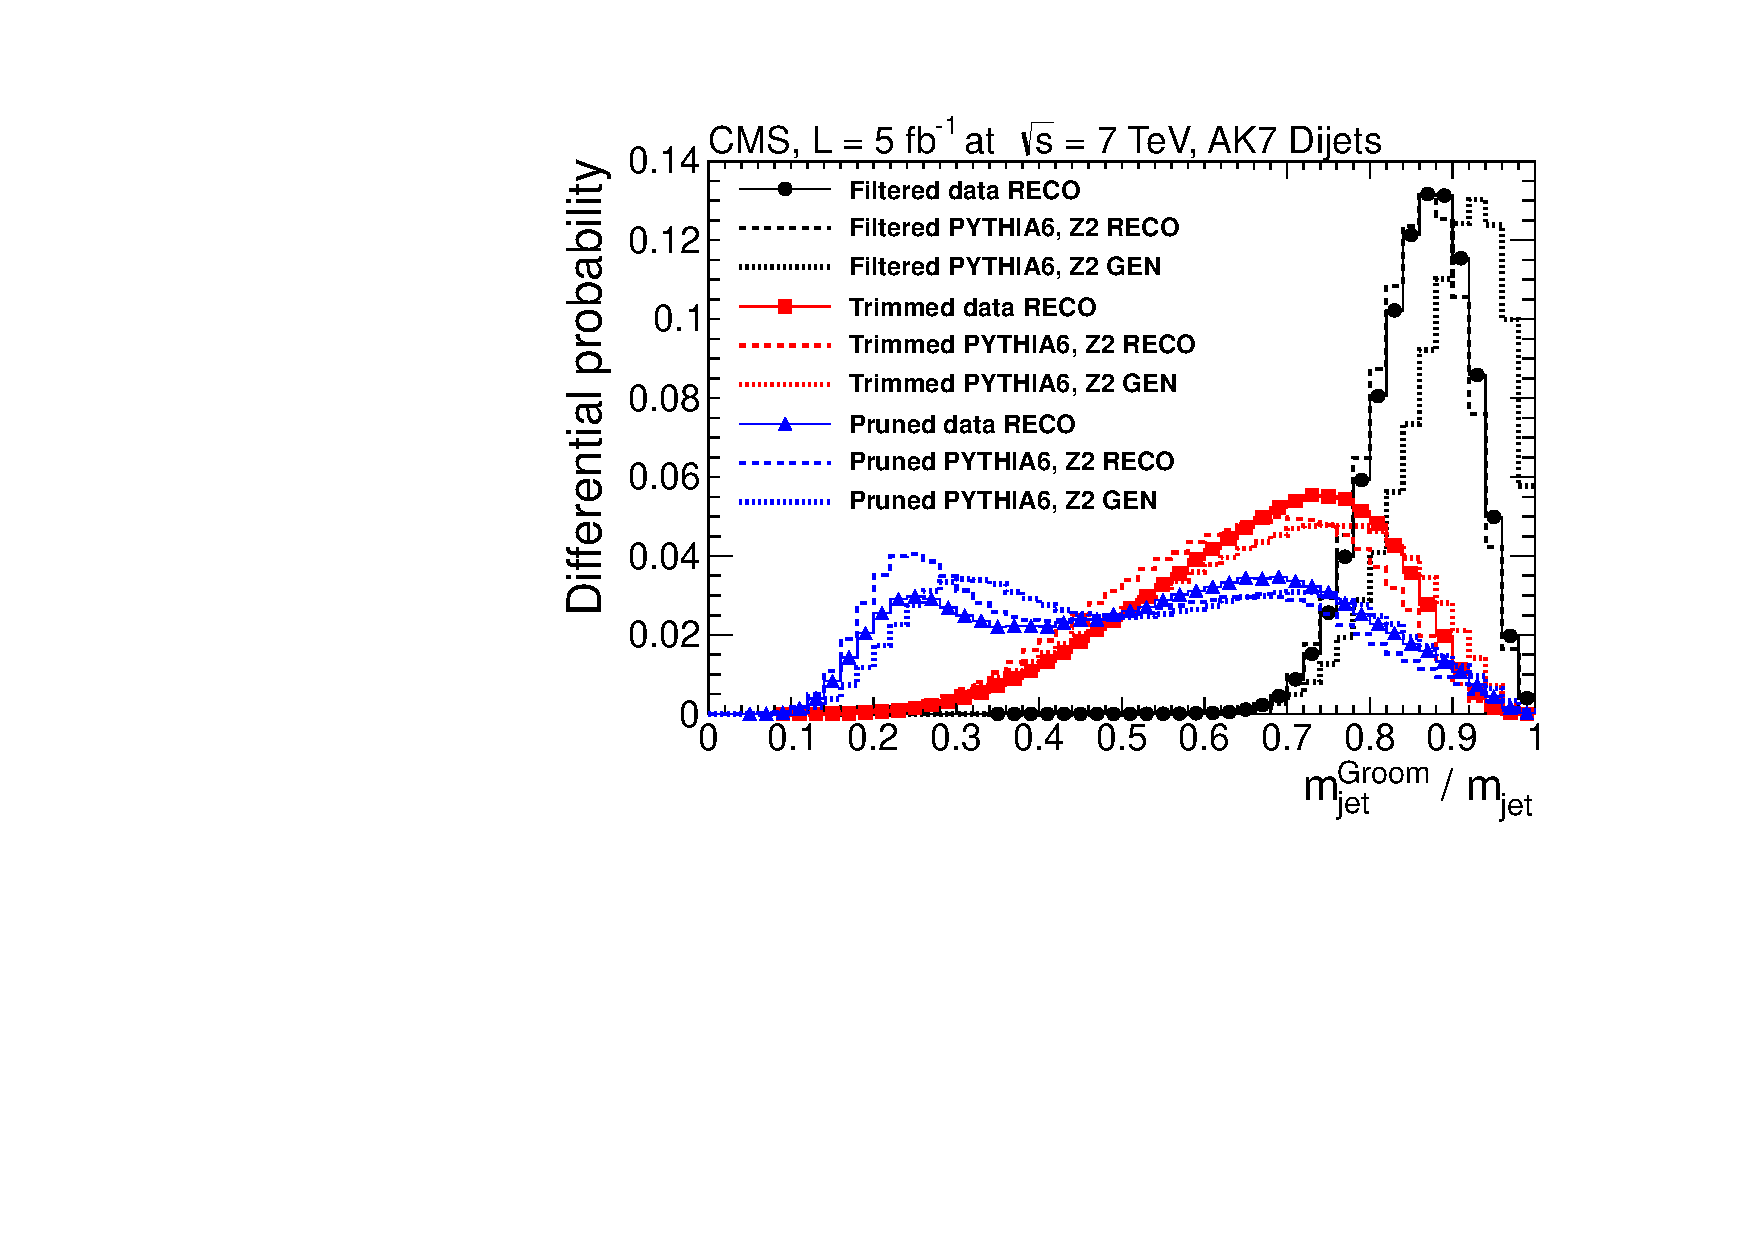
\includegraphics[width=0.95\textwidth]{figs/histAK7PtAvgVsMjetGroomOverReco_ratioPlots}
\caption{Distributions in differential probability for ratios of the jet mass of groomed jets
to their
corresponding ungroomed values, for both dijet data and \PYTHIA (tune Z2) MC
simulation, for the
three grooming techniques discussed in the text: 
(i) filtering (circles, peaking near $0.9$), 
(ii) trimming (squares, peaking near $0.75$), and 
(iii) pruning (triangles, more dispersed). 
\label{figs:histAK7PtAvgVsMjetGroomOverReco_ratioPlots}}
\end{figure}





